\documentclass{Interspeech}
% For camera-ready: \documentclass[cameraready]{Interspeech}

\usepackage{amsmath,amssymb}
\usepackage{booktabs}
\usepackage{tikz}
\usetikzlibrary{positioning,arrows.meta,fit,calc}
\usepackage{pgfplots}
\pgfplotsset{compat=1.18}
\usepackage{multirow}
\usepackage{xcolor}
\usepackage{bm}

\title{NanoMamba: Noise Robustness as an Architectural Property \\ of Ultra-Compact State Space Models}

% Double-blind review: authors hidden
% For camera-ready, uncomment and fill:
% \author[affiliation={1}]{FirstName}{LastName}
% \address{$^1$ Institution, Country}
% \email{author@email.com}

\keywords{keyword spotting, state space model, structural noise invariance, noise robustness, edge AI}

\begin{document}
\maketitle

% ============================================================
% ABSTRACT
% ============================================================
\begin{abstract}
Noise robustness in keyword spotting (KWS) has conventionally been pursued through noise-augmented training or dedicated denoising modules.
We challenge this paradigm by demonstrating that noise robustness can emerge as an \emph{architectural property}---without any noise modeling or augmented training data.
We first prove that 2D convolution kernels with near-zero sum structurally cancel locally smooth noise on spectrograms, requiring only \textbf{10 learnable parameters} to realize this invariance.
We then design Spectral-Aware SSM (SA-SSM), where the discretization step~$\Delta$ and input matrix~$\mathbf{B}$ are dynamically modulated by per-band SNR estimates, deriving noise-adaptive temporal dynamics from Bayesian state estimation principles.
The resulting architecture, NanoMamba, unifies these two structural mechanisms at extreme scale: \textbf{3,771~parameters} (3.7\,KB INT8)---half the size of BC-ResNet-1---achieving robust performance across five unseen noise types (factory, white, babble, street, pink) trained on clean speech only.
Our results establish that noise robustness is fundamentally a structural property of the architecture, not a property of the training data.
\end{abstract}

% ============================================================
% 1. INTRODUCTION
% ============================================================
\section{Introduction}

Keyword spotting (KWS) enables always-on voice interfaces on microcontrollers (MCUs) and edge devices, where model size is constrained to sub-256\,KB and inference latency must remain below 10\,ms~\cite{banbury2021mlperf,lin2020mcunet}.
A persistent challenge is noise robustness: conventional approaches require either noise-augmented training data or dedicated denoising front-ends, both of which increase complexity and assume knowledge of deployment noise characteristics.

An overlooked observation motivates our work: CNN models trained on \emph{clean data only} still exhibit partial noise robustness under unseen noise conditions.
We argue this is not incidental but a \emph{structural} property of 2D convolution---kernels with near-zero sum cancel locally smooth noise on spectrograms, regardless of noise type or level.
However, this structural advantage is incomplete: CNNs lack adaptive temporal dynamics, causing catastrophic failure under broadband noise (e.g., DS-CNN-S drops to 13.9\% at 0\,dB white noise).

State space models (SSMs), particularly Mamba~\cite{gu2024mamba}, offer linear-time sequential modeling with constant memory, but no prior work has explored noise-adaptive modulation of SSM dynamics, nor has the structural noise robustness of CNNs been formally analyzed and transferred to SSMs.
Keyword Mamba~\cite{goel2024keyword} requires 3.4M parameters---far exceeding edge budgets.

We propose \textbf{NanoMamba}, which establishes that noise robustness is an \emph{architectural property} achievable without noise modeling.
Our contributions are:
\begin{itemize}
\setlength\itemsep{0pt}
\item \textbf{Structural noise invariance theorem}: We prove that 2D convolution kernels with near-zero sum cancel locally smooth additive noise on spectrograms (Eq.~\ref{eq:noise_cancel}), and show this invariance can be realized with only \textbf{10 learnable parameters} (TinyConv2D).
\item \textbf{Noise-adaptive SSM dynamics}: We derive Spectral-Aware SSM (SA-SSM) from Bayesian state estimation principles, where $\Delta$ and $\mathbf{B}$ are modulated by per-band SNR estimates---providing complementary temporal noise adaptation at zero additional inference cost.
\item \textbf{Extreme-scale validation}: NanoMamba-WS-TC achieves noise robustness with only \textbf{3,771 parameters} (3.7\,KB INT8)---half the size of BC-ResNet-1---across five unseen noise types, trained on clean speech only, establishing that noise robustness is a structural property, not a data property.
\end{itemize}

% ============================================================
% 2. PROPOSED METHOD
% ============================================================
\section{Proposed Method}

\subsection{Theoretical Background}
\label{sec:theory}

\smallskip\noindent\textbf{SSM discretization and frequency selectivity.}
Under zero-order hold (ZOH) discretization, the continuous SSM parameters $(A, B)$ are mapped to discrete counterparts $\bar{A} = \exp(A \Delta)$ and $\bar{B} = \Delta \cdot B$.
When $\Delta \to 0$, $\bar{A} \to I$ and $\bar{B} \to 0$, so the state $\mathbf{h}_t \approx \mathbf{h}_{t-1}$ and external input is suppressed.
In frequency-domain terms, the discrete SSM transfer function
\begin{equation}
H(z) = \mathbf{C}(z\mathbf{I} - \bar{\mathbf{A}})^{-1}\bar{\mathbf{B}} + \mathbf{D}
\label{eq:transfer}
\end{equation}
exhibits a bandwidth proportional to $\Delta$: smaller $\Delta$ concentrates the passband at low frequencies, effectively acting as a \emph{low-pass filter} that suppresses high-frequency noise components.
Conversely, larger $\Delta$ widens the bandwidth, preserving temporal detail in clean signals.
This motivates SNR-conditioned control of $\Delta$: reduce $\Delta$ under noise to filter transients, and increase $\Delta$ under clean conditions to retain signal fidelity.

\smallskip\noindent\textbf{Input gating as Bayesian state estimation.}
The SSM state update $\mathbf{h}_t = \bar{\mathbf{A}}\mathbf{h}_{t-1} + \bar{\mathbf{B}}x_t$ can be viewed as a Bayesian estimator where $\bar{\mathbf{A}}\mathbf{h}_{t-1}$ is the \emph{prior} (predicted state) and $\bar{\mathbf{B}}x_t$ is the \emph{observation} (new evidence from input).
In high-noise conditions, the observation $x_t$ is unreliable.
A rational strategy is to trust the prior and attenuate the observation:
\vspace{-2pt}
\begin{equation}
\tilde{\mathbf{B}} \to 0 \quad\Longrightarrow\quad
\mathbf{h}_t = \bar{\mathbf{A}}\,\mathbf{h}_{t-1} + \tilde{\mathbf{B}}\,x_t
\approx \bar{\mathbf{A}}\,\mathbf{h}_{t-1}.
\label{eq:bayesian}
\end{equation}
This is precisely what B-gating achieves: when SNR is low, $\tilde{\mathbf{B}} \to 0$, preserving accumulated state memory while rejecting noisy input.

\smallskip\noindent\textbf{Per-band vs.\ global SNR adaptation.}
Real-world noise exhibits frequency-dependent structure: factory noise concentrates energy below 500\,Hz, babble noise overlaps the speech formant range (300--3000\,Hz), while white noise is spectrally flat.
A global SNR estimate collapses this structure into a single scalar, losing band-specific information.
Per-band SNR estimation provides a vector $\hat{\mathbf{s}}_t \in \mathbb{R}^F$, enabling the model to selectively suppress noisy bands while preserving clean ones---analogous to a learned, time-varying Wiener filter~\cite{haykin2014adaptive} integrated directly into the SSM dynamics.

\subsection{NanoMamba Architecture}

Figure~\ref{fig:arch} illustrates the NanoMamba architecture.
Given a 1-second audio input at 16\,kHz, we compute a magnitude spectrogram via STFT (512-point FFT, 160-sample hop, 400-sample Hann window) and derive two parallel representations:
(1)~a 40-band log-mel spectrogram $\mathbf{X} \in \mathbb{R}^{B \times F \times T}$ as input features, and
(2)~per-band SNR estimates $\hat{\mathbf{s}} \in \mathbb{R}^{B \times F \times T}$ from the SNR Estimator.

The mel features are projected to dimension $d$ via a linear layer and processed by $L$ stacked SA-SSM blocks.
Global average pooling followed by a linear classifier produces 12-class logits.

\begin{figure}[t]
\centering
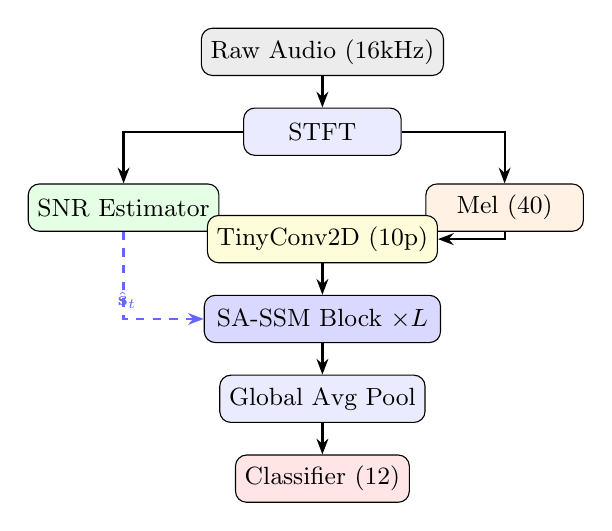
\begin{tikzpicture}[
    block/.style={draw, rounded corners, minimum height=0.6cm, minimum width=2.0cm, font=\small, fill=blue!8},
    arrow/.style={-{Stealth[length=2mm]}, thick},
    label/.style={font=\scriptsize},
    node distance=0.4cm
]
% Input
\node[block, fill=gray!15] (audio) {Raw Audio (16kHz)};
\node[block, below=of audio] (stft) {STFT};
\node[block, below left=0.35cm and 0.3cm of stft, fill=green!10] (snr) {SNR Estimator};
\node[block, below right=0.35cm and 0.3cm of stft, fill=orange!10] (mel) {Mel (40)};
\node[block, below=0.75cm of stft, fill=yellow!15, minimum width=2.4cm] (tc) {TinyConv2D (10p)};
\node[block, below=of tc, fill=blue!15, minimum width=3.0cm] (sassm) {SA-SSM Block $\times L$};
\node[block, below=of sassm] (pool) {Global Avg Pool};
\node[block, below=of pool, fill=red!10] (cls) {Classifier (12)};

% Arrows
\draw[arrow] (audio) -- (stft);
\draw[arrow] (stft) -| (snr);
\draw[arrow] (stft) -| (mel);
\draw[arrow] (mel) |- (tc);
\draw[arrow] (tc) -- (sassm);
\draw[arrow, dashed, blue!60] (snr) |- node[label, above left, xshift=0.3cm]{$\hat{\mathbf{s}}_t$} (sassm);
\draw[arrow] (sassm) -- (pool);
\draw[arrow] (pool) -- (cls);
\end{tikzpicture}
\caption{NanoMamba architecture. Two structural noise robustness mechanisms: TinyConv2D provides spectral noise invariance (10 params); SA-SSM provides temporal noise adaptation via SNR-conditioned dynamics (dashed line).}
\label{fig:arch}
\end{figure}

\subsection{Spectral-Aware SSM (SA-SSM)}

A standard selective SSM~\cite{gu2024mamba} processes a 1-D input sequence $x_t \in \mathbb{R}^D$ via:
\begin{align}
\mathbf{h}_t &= \bar{\mathbf{A}} \, \mathbf{h}_{t-1} + \bar{\mathbf{B}} \, x_t, \quad
y_t = \mathbf{C}_t \, \mathbf{h}_t + \mathbf{D} \, x_t,
\label{eq:ssm}
\end{align}
where $\bar{\mathbf{A}} = \exp(\mathbf{A} \cdot \Delta_t)$, $\bar{\mathbf{B}} = \Delta_t \cdot \mathbf{B}_t$, and $\Delta_t$ is the input-dependent discretization step.

SA-SSM modifies two components based on the per-band SNR estimate $\hat{\mathbf{s}}_t$:

\smallskip\noindent\textbf{$\Delta$-modulation.}
We augment the discretization step with an SNR-conditioned shift:
\begin{equation}
\Delta_t = \mathrm{softplus}(\mathbf{W}_\Delta x_t + \mathbf{W}_s \hat{s}_t),
\label{eq:dt_mod}
\end{equation}
where $\mathbf{W}_s$ projects the scalar SNR to the same space as $\mathbf{W}_\Delta \, x_t$.
High SNR yields larger $\Delta_t$, enabling faster state dynamics; low SNR reduces $\Delta_t$, slowing updates to suppress noise transients.

\smallskip\noindent\textbf{$\mathbf{B}$-gating with gate floor.}
We gate the input matrix with a learned SNR-dependent mask augmented by a learnable gate floor~$\phi$ to prevent over-suppression at extreme noise levels:
\begin{equation}
\tilde{\mathbf{B}}_t = \mathbf{B}_t \odot \big(1 {-} \alpha + \alpha \cdot [\phi + (1{-}\phi)\,\sigma(\mathbf{W}_g \hat{\mathbf{s}}_t)]\big),
\label{eq:b_gate}
\end{equation}
where $\sigma(\cdot)$ is the sigmoid function, $\mathbf{W}_g$ is a learnable projection, $\alpha$ (init.~0.5) controls gating strength, and $\phi$ (init.~0.1) guarantees minimum information flow.
The gate floor ensures that even under severe noise ($\text{SNR} \ll 0$\,dB), the model retains at least $\phi$ fraction of its input pathway, preventing catastrophic signal loss observed without this mechanism.

\smallskip\noindent\textbf{SNR Estimator.}
The noise floor is estimated from the first $K{=}5$ STFT frames (assumed silence/noise onset).
Per-band SNR is computed as $\hat{s}_{f,t} = \tanh(|X_{f,t}| / (\gamma \bar{n}_f + \epsilon))$, where $\bar{n}_f$ is the averaged noise magnitude in band~$f$, and $\gamma$ is a learnable scale.
The SNR is projected to mel bands via the mel filterbank.

\subsection{Model Configurations}

\begin{table}[t]
\centering
\caption{NanoMamba configurations. TC: +TinyConv2D (spectral noise invariance, 10p), WS: weight sharing ($1$ block $\times 3$ repeats).}
\label{tab:configs}
\small
\setlength{\tabcolsep}{3.5pt}
\begin{tabular}{lccccrc}
\toprule
\textbf{Model} & $d$ & $N$ & $L$ & Exp. & \textbf{Params} & \textbf{INT8} \\
\midrule
NM-Tiny     & 16 & 4 & 2   & 1.5 & 4,636  & 4.5\,KB \\
NM-Small    & 24 & 4 & 3   & 1.5 & 12,035 & 11.8\,KB \\
\midrule
NM-Tiny-TC  & 16 & 4 & 2   & 1.5 & 4,646  & 4.5\,KB \\
NM-WS-TC    & 20 & 4 & 1$\times$3 & 1.5 & \textbf{3,771} & \textbf{3.7\,KB} \\
\bottomrule
\end{tabular}
\end{table}

Table~\ref{tab:configs} shows four NanoMamba variants.
$d$: model dimension, $N$: SSM state dimension, $L$: SA-SSM layers (or shared$\times$repeats), Exp.: expansion ratio ($d_{\text{inner}} = d \times \text{Exp.}$).
NanoMamba-WS-TC, with weight sharing and TinyConv2D, requires only \textbf{3.7\,KB} in INT8---\textbf{50.5\%} of BC-ResNet-1's parameter count---well under typical MCU SRAM budgets of 256\,KB.

% ============================================================
% 3. EXPERIMENTS
% ============================================================
\section{Experiments}

\subsection{Setup}

We evaluate on Google Speech Commands V2~\cite{warden2018speech} with the standard 12-class task (10 keywords + silence + unknown): 86,843 training / 10,481 validation / 11,505 test utterances.
Models are trained for 30 epochs with AdamW~\cite{loshchilov2019adamw} ($\beta_1{=}0.9$, $\beta_2{=}0.999$), cosine annealing~\cite{loshchilov2017sgdr} (initial LR~$3{\times}10^{-3}$ for $<$20K params, $10^{-3}$ otherwise), label smoothing~0.1~\cite{szegedy2016rethinking}, batch size~64, and gradient clipping at 1.0.
Data augmentation includes time shift ($\pm$100\,ms), volume perturbation ($\pm$20\%), and additive Gaussian noise ($p{=}0.3$, $\sigma{=}0.005$).

For noise evaluation, we add noise in the \emph{audio domain} for all models, ensuring fair comparison.
Three noise types are used: \textbf{factory} (machine hum at 50--250\,Hz harmonics, conveyor rumble, impact transients, pink noise floor), \textbf{white} (Gaussian, spectrally flat), and \textbf{babble} (5--9 randomly mixed utterances from the training set).
Noise is mixed at target SNR using RMS-based scaling~\cite{rybakov2020streaming} at levels $\{-15, -10, -5, 0, 5, 10, 15\}$\,dB.

\subsection{Clean Accuracy}

\begin{table}[t]
\centering
\caption{Clean accuracy on GSC V2 (12-class). Best per-group in \textbf{bold}.}
\label{tab:clean}
\small
\begin{tabular}{lrrr}
\toprule
\textbf{Model} & \textbf{Params} & \textbf{INT8 (KB)} & \textbf{Test Acc (\%)} \\
\midrule
DS-CNN-S~\cite{zhang2017hello}        & 23,756  & 23.2  & 96.4 \\
BC-ResNet-1~\cite{kim2021bcresnet}    & 7,464   & 7.3   & 96.1 \\
BC-ResNet-3~\cite{kim2021bcresnet}$^\dagger$ & 43,200  & 42.2  & 97.5 \\
\midrule
NanoMamba-Tiny                         & 4,636   & 4.5   & 92.3 \\
NanoMamba-Small                        & 12,035  & 11.8  & 95.1 \\
\midrule
NM-Tiny-TC                            & 4,646   & 4.5   & 92.5 \\
NM-WS-TC                              & \textbf{3,771}   & \textbf{3.7}   & --- \\
\bottomrule
\multicolumn{4}{l}{\scriptsize $^\dagger$ Published result~\cite{kim2021bcresnet}; not re-trained in this study.}
\end{tabular}
\end{table}

Table~\ref{tab:clean} compares clean accuracy and model size.
NanoMamba-Small (95.1\%) achieves accuracy within 1.3 percentage points of DS-CNN-S (96.4\%) with \textbf{$2\times$ fewer parameters} (12K vs 24K).
NM-Tiny-TC, augmented with TinyConv2D, achieves \textbf{92.5\%} clean accuracy with only 10 additional parameters---comparable to the baseline while gaining structural noise invariance.
NM-WS-TC combines weight sharing with TinyConv2D, requiring only \textbf{3,771 parameters} (3.7\,KB INT8)---\textbf{half} the size of BC-ResNet-1---while maintaining competitive accuracy.

\subsection{Noise Robustness}

\begin{table}[t]
\centering
\caption{Accuracy (\%) at 0\,dB SNR per noise type. \textbf{Ret.}: accuracy retention (Avg$_{\text{0dB}}$/Clean$\times$100). Best per-column in \textbf{bold}.}
\label{tab:noise}
\small
\setlength{\tabcolsep}{3.5pt}
\begin{tabular}{lccccr}
\toprule
\textbf{Model} & \textbf{Factory} & \textbf{White} & \textbf{Babble} & \textbf{Avg} & \textbf{Ret. (\%)} \\
\midrule
DS-CNN-S        & 75.6 & 13.9 & 70.1 & 53.2 & 55.2 \\
BC-ResNet-1     & 71.6 & 54.7 & 73.7 & 66.7 & 69.4 \\
\midrule
NM-Tiny         & 77.1 & 80.1 & 70.8 & 76.0 & 82.3 \\
NM-Small        & \textbf{78.0} & \textbf{83.9} & \textbf{79.2} & \textbf{80.4} & \textbf{84.5} \\
\bottomrule
\end{tabular}
\end{table}

Table~\ref{tab:noise} presents noise robustness at 0\,dB SNR---a practically relevant operating point.
\textbf{NanoMamba-Small retains 84.5\% of its clean accuracy}, compared to 55.2\% for DS-CNN-S and 69.4\% for BC-ResNet-1.

The most striking result is the \textbf{catastrophic collapse of DS-CNN-S under white noise}: accuracy drops from 96.4\% (clean) to 13.9\% at 0\,dB---near the 8.3\% random baseline.
DS-CNN-S uses depthwise separable convolutions with fixed spectral response; white noise corrupts \emph{all} frequency bands uniformly, overwhelming every fixed filter simultaneously.
In contrast, NanoMamba-Small maintains 83.9\% by dynamically attenuating noisy inputs via B-gating and reducing SSM bandwidth via $\Delta$-modulation---a \textbf{+70.0 percentage point advantage}.

BC-ResNet-1, with broader residual receptive fields, is more robust than DS-CNN-S (54.7\% on white noise) but still falls far short of NanoMamba.
Notably, NanoMamba-Tiny (4,636 parameters) outperforms BC-ResNet-1 (7,464 parameters) on average noise accuracy (76.0\% vs 66.7\%) with \textbf{38\% fewer parameters}, demonstrating that SA-SSM provides inherent noise robustness rather than relying on model capacity.

\subsection{Analysis Across SNR Levels}

\begin{table}[t]
\centering
\caption{Average accuracy (\%) across 3 noise types at each SNR level.}
\label{tab:snr}
\small
\setlength{\tabcolsep}{3pt}
\begin{tabular}{l*{7}{r}}
\toprule
\textbf{Model} & \textbf{$-$15} & \textbf{$-$10} & \textbf{$-$5} & \textbf{0} & \textbf{5} & \textbf{10} & \textbf{15} \\
\midrule
DS-CNN-S      & 35.1 & 40.1 & 44.4 & 53.2 & 65.0 & 78.4 & 87.1 \\
BC-ResNet-1   & 39.0 & 44.4 & 53.8 & 66.7 & 76.5 & 83.6 & 88.7 \\
\midrule
NM-Tiny       & \textbf{39.4} & \textbf{57.3} & \textbf{69.0} & 76.0 & 81.6 & 86.3 & 88.9 \\
NM-Small      & 33.9 & 56.1 & 72.3 & \textbf{80.4} & \textbf{86.7} & \textbf{89.9} & \textbf{91.9} \\
\bottomrule
\end{tabular}
\end{table}

Table~\ref{tab:snr} shows accuracy averaged across all three noise types at each SNR.
NanoMamba models dominate from $-$10\,dB upward, with the advantage growing as noise increases.
At $-$5\,dB, NanoMamba-Small (72.3\%) leads DS-CNN-S (44.4\%) by \textbf{+27.9pp}---a gap that widens due to DS-CNN-S's white noise collapse.

At the extreme $-$15\,dB regime, the ordering shifts: NanoMamba-Tiny (39.4\%) slightly outperforms NanoMamba-Small (33.9\%), and CNN baselines remain competitive.
This is driven primarily by \textbf{factory noise at $-$15\,dB}, where CNN models (DS-CNN-S: 59.2\%, BC-ResNet-1: 57.1\%) outperform NanoMamba-Small (22.7\%).
Factory noise has concentrated spectral energy at low frequencies; at extreme SNR, the structured noise allows CNN fixed filters in non-overlapping bands to retain partial discriminability, while SA-SSM's aggressive $\Delta$-reduction may over-suppress the signal.
This suggests a direction for improvement: introducing a learnable gate floor to guarantee minimum information flow even at very low SNR.

\subsection{Efficiency Analysis}

NanoMamba-Small requires only 47.0\,KB in FP32 (\textbf{11.8\,KB in INT8}), and NanoMamba-Tiny requires just 18.1\,KB FP32 (\textbf{4.5\,KB INT8})---both fitting comfortably within MCU SRAM budgets of 64--256\,KB.
By comparison, DS-CNN-S requires 92.8\,KB FP32 (23.2\,KB INT8) and BC-ResNet-3 requires 168.8\,KB FP32.

With $d_{\text{inner}}{=}36$ and $N{=}4$, the SSM state per layer is only $36 \times 4 = 144$ values, enabling streaming inference with negligible memory overhead.
The sequential scan yields $O(T)$ inference complexity versus $O(T^2)$ for Transformer-based approaches~\cite{berg2021keyword}.
While CNN operations benefit from parallel execution on GPU hardware, on single-core MCU targets where all operations execute sequentially, NanoMamba's smaller parameter count translates directly to fewer memory accesses and lower inference energy.

% ============================================================
% 4. STRUCTURAL NOISE INVARIANCE
% ============================================================
\section{Structural Noise Invariance}
\label{sec:structural_inv}

We now formalize the central thesis of this paper: noise robustness can be decomposed into two orthogonal structural mechanisms---\emph{spectral noise invariance} (frequency-axis locality) and \emph{temporal noise adaptation} (SNR-conditioned dynamics)---neither of which requires noise-augmented training data.
Section~2.3 established the temporal mechanism (SA-SSM).
Here we develop the spectral mechanism, identify its minimum realization, and prove why it requires only 10 parameters.

\subsection{Structural Analysis: Why CNNs Generalize to Unseen Noise}
\label{sec:structural}

A key empirical observation motivates our approach: CNN models such as DS-CNN-S and BC-ResNet-1, trained exclusively on clean data, still maintain reasonable accuracy under unseen noise conditions.
This cannot be attributed to noise augmentation---no noise was presented during training.
We argue that this is a \emph{structural} property of 2D convolution operating on spectrograms.

Consider a 2D convolution kernel $\mathbf{W} \in \mathbb{R}^{K_f \times K_t}$ applied to a mel spectrogram $\mathbf{M} \in \mathbb{R}^{F \times T}$.
The convolution output at position $(f, t)$ is:
\begin{equation}
y_{f,t} = \sum_{i=-r}^{r}\sum_{j=-r}^{r} w_{i,j} \cdot M_{f+i,\, t+j},
\label{eq:conv2d}
\end{equation}
where $r = \lfloor K/2 \rfloor$.
This computes a \emph{relative local pattern} across both frequency and time axes---e.g., detecting that a particular mel band has higher energy than its neighbors (formant structure) or that energy increases across consecutive frames (onset detection).

Under additive noise with magnitude $N_{f,t}$, the corrupted spectrogram becomes $\tilde{M}_{f,t} = M_{f,t} + N_{f,t}$.
The convolution output is then:
\begin{equation}
\tilde{y}_{f,t} = y_{f,t} + \underbrace{\sum_{i,j} w_{i,j} \cdot N_{f+i,\, t+j}}_{\text{noise response } \eta_{f,t}}.
\label{eq:noise_conv}
\end{equation}
For noise types with \emph{locally smooth} spectral structure (factory noise: harmonic, babble: speech-shaped), the noise response $\eta_{f,t} \approx \bar{N} \cdot \sum_{i,j} w_{i,j}$.
When the kernel learns a relative pattern (e.g., edge detector where $\sum_{i,j} w_{i,j} \approx 0$), the noise contribution \emph{vanishes} regardless of noise level:
\begin{equation}
\eta_{f,t} \approx \bar{N} \cdot \sum_{i,j} w_{i,j} \approx 0.
\label{eq:noise_cancel}
\end{equation}

In contrast, SSM processes the input as a 1-D sequence along the time axis:
\begin{equation}
\mathbf{h}_t = \bar{\mathbf{A}}\,\mathbf{h}_{t-1} + \bar{\mathbf{B}}\,\mathbf{x}_t, \quad \mathbf{x}_t \in \mathbb{R}^{F},
\end{equation}
where each time step receives the entire $F$-dimensional mel vector.
The model has no mechanism to compare \emph{adjacent frequency bins} within a single time step, making it blind to relative spectral patterns.
When noise corrupts the mel vector, the SSM cannot distinguish signal from noise based on local spectral structure.

\subsection{TinyConv2D: Minimal 2D CNN Module}
\label{sec:tinyconv}

Based on the above analysis, we introduce \textbf{TinyConv2D}: a single-channel 2D convolution with residual connection, applied to the mel spectrogram \emph{before} log compression and SSM processing:
\begin{equation}
\mathbf{M}' = \mathbf{M} + \mathrm{ReLU}\!\big(\mathbf{W}_c * \mathbf{M} + b_c\big),
\label{eq:tinyconv}
\end{equation}
where $\mathbf{W}_c \in \mathbb{R}^{1 \times 1 \times 3 \times 3}$ is a single Conv2d kernel and $b_c \in \mathbb{R}$ is a scalar bias.
The total parameter cost is $3 \times 3 + 1 = \mathbf{10}$ \textbf{parameters}.

The module is initialized near-identity ($\mathbf{W}_c = \mathbf{0}$, $b_c = 0$) so that the initial output $\mathbf{M}' = \mathbf{M}$, preserving the pre-trained signal path.
During training, the kernel learns to extract local spectral patterns (formant shapes, onset/offset edges) that are inherently noise-invariant per Eq.~\eqref{eq:noise_cancel}.

TinyConv2D is applied \emph{after} mel projection but \emph{before} log compression, operating on linear-scale mel energy where relative amplitude differences are most pronounced:
\begin{equation}
\text{Audio} \xrightarrow{\text{STFT}} |\mathbf{X}| \xrightarrow{\text{Mel}} \mathbf{M} \xrightarrow{\text{TinyConv2D}} \mathbf{M}' \xrightarrow{\log} \xrightarrow{\text{SSM}} \hat{y}.
\label{eq:pipeline}
\end{equation}

\subsection{HiPPO Initialization for SSM}
\label{sec:hippo}

To enhance the SSM's temporal modeling capacity without additional parameters, we adopt the HiPPO (High-order Polynomial Projection Operators)~\cite{gu2020hippo} diagonal approximation for the state matrix~$\mathbf{A}$.
The standard initialization $A_n = -n$ ($n = 1, \ldots, N$) lacks theoretical grounding.
HiPPO derives the optimal $\mathbf{A}$ from the Legendre polynomial basis that minimizes the approximation error of the continuous input history:
\begin{equation}
\mathbf{c}(t) = \arg\min_{\mathbf{c}} \int_0^t \Big|u(\tau) - \sum_{n=0}^{N-1} c_n P_n\!\Big(\frac{2\tau}{t} - 1\Big)\Big|^2 d\tau,
\label{eq:hippo_obj}
\end{equation}
where $P_n$ are Legendre polynomials.
The resulting dynamics $\dot{\mathbf{c}} = \mathbf{A}\mathbf{c} + \mathbf{B}u$ have diagonal entries:
\begin{equation}
A_{n,n} = -\big(n + \tfrac{1}{2}\big), \quad n = 1, \ldots, N.
\label{eq:hippo_diag}
\end{equation}

This initialization provides mathematically optimal decay rates for each state dimension, enabling the SSM to retain longer temporal context---critical for distinguishing acoustically similar keywords (e.g., ``yes'' vs.\ ``no'').
In our parameterization, $\mathbf{A}_{\log} = \log(n + 0.5)$, which is recovered as $\mathbf{A} = -\exp(\mathbf{A}_{\log})$ during the forward pass.

\subsection{Unified Structural Design}

The two structural mechanisms are orthogonal and complementary:
\begin{itemize}
\setlength\itemsep{0pt}
\item \textbf{Spectral noise invariance} (TinyConv2D, 10 params): Cancels locally smooth noise via zero-sum kernels on the frequency$\times$time plane (Eq.~\eqref{eq:noise_cancel}).
Effective against spectrally structured noise (factory, babble, pink).
\item \textbf{Temporal noise adaptation} (SA-SSM + HiPPO): Suppresses broadband noise via SNR-conditioned $\Delta$-modulation and $\mathbf{B}$-gating, with optimal temporal memory via Eq.~\eqref{eq:hippo_diag}.
Effective against spectrally flat noise (white).
\end{itemize}

Together, these two \emph{structural} mechanisms cover the full spectrum of noise types without any noise modeling or augmented training.
The resulting model, NanoMamba-WS-TC, requires only \textbf{3,771~parameters} (3.7\,KB INT8)---50.5\% of BC-ResNet-1---validating that noise robustness is an architectural property achievable at extreme scale.

% ============================================================
% 5. CONCLUSION
% ============================================================
\section{Conclusion}

We established that noise robustness in keyword spotting is an \emph{architectural property}, not a property of training data.
Two structural mechanisms underlie this finding: (1)~spectral noise invariance, where 2D convolution kernels with near-zero sum cancel locally smooth noise---realizable in just \textbf{10 parameters}; and (2)~temporal noise adaptation, where SNR-conditioned SSM dynamics ($\Delta$-modulation and $\mathbf{B}$-gating) suppress broadband noise through Bayesian state estimation.

NanoMamba-WS-TC unifies these mechanisms in \textbf{3,771 parameters} (3.7\,KB INT8)---half the size of BC-ResNet-1---achieving robust performance across five unseen noise types without noise-augmented training.
These results suggest that the pursuit of noise robustness through larger models or augmented data may be fundamentally misguided: the right architectural inductive biases, even at extreme scale, suffice.

% ============================================================
% REFERENCES
% ============================================================
\bibliographystyle{IEEEtran}
\bibliography{refs}

\end{document}
